\chapter{Dashboards}

Los paneles de información (en inglés \textit{dashboard}) son herramientas gráficas que nos permiten visualizar datos para convertirlos en información sin tener que realizar ningún tipo de programación.

Podríamos decir que los paneles son un interfaz gráfico previamente programado que obtiene datos de una fuente de datos (una hoja de cálculo, un fichero CSV, una base de datos,...) para posteriormente visualizarlo de una forma gráfica.

\chapter{Características}

Los paneles de información suelen contar con las siguientes características:

\begin{itemize}
    \item Son \textbf{fáciles de usar}: no es necesario ser programador para hacer uso de ellos, \textbf{siempre y cuando los datos los tengamos en un formato correcto}.
    \item Permiten hacer uso de \textbf{diferentes tipos de gráficos}: tablas, mapas para datos geolocalizados, mapas de calor, gráficos tipo tarta, mapas de barras (horizontales y verticales), ...

    \item Son \textbf{interactivos}: podemos hacer que los gráficos estén enlazados entre sí, y de esta manera al seleccionar un apartado de uno, el resto se actualizan.

    \begin{center}
        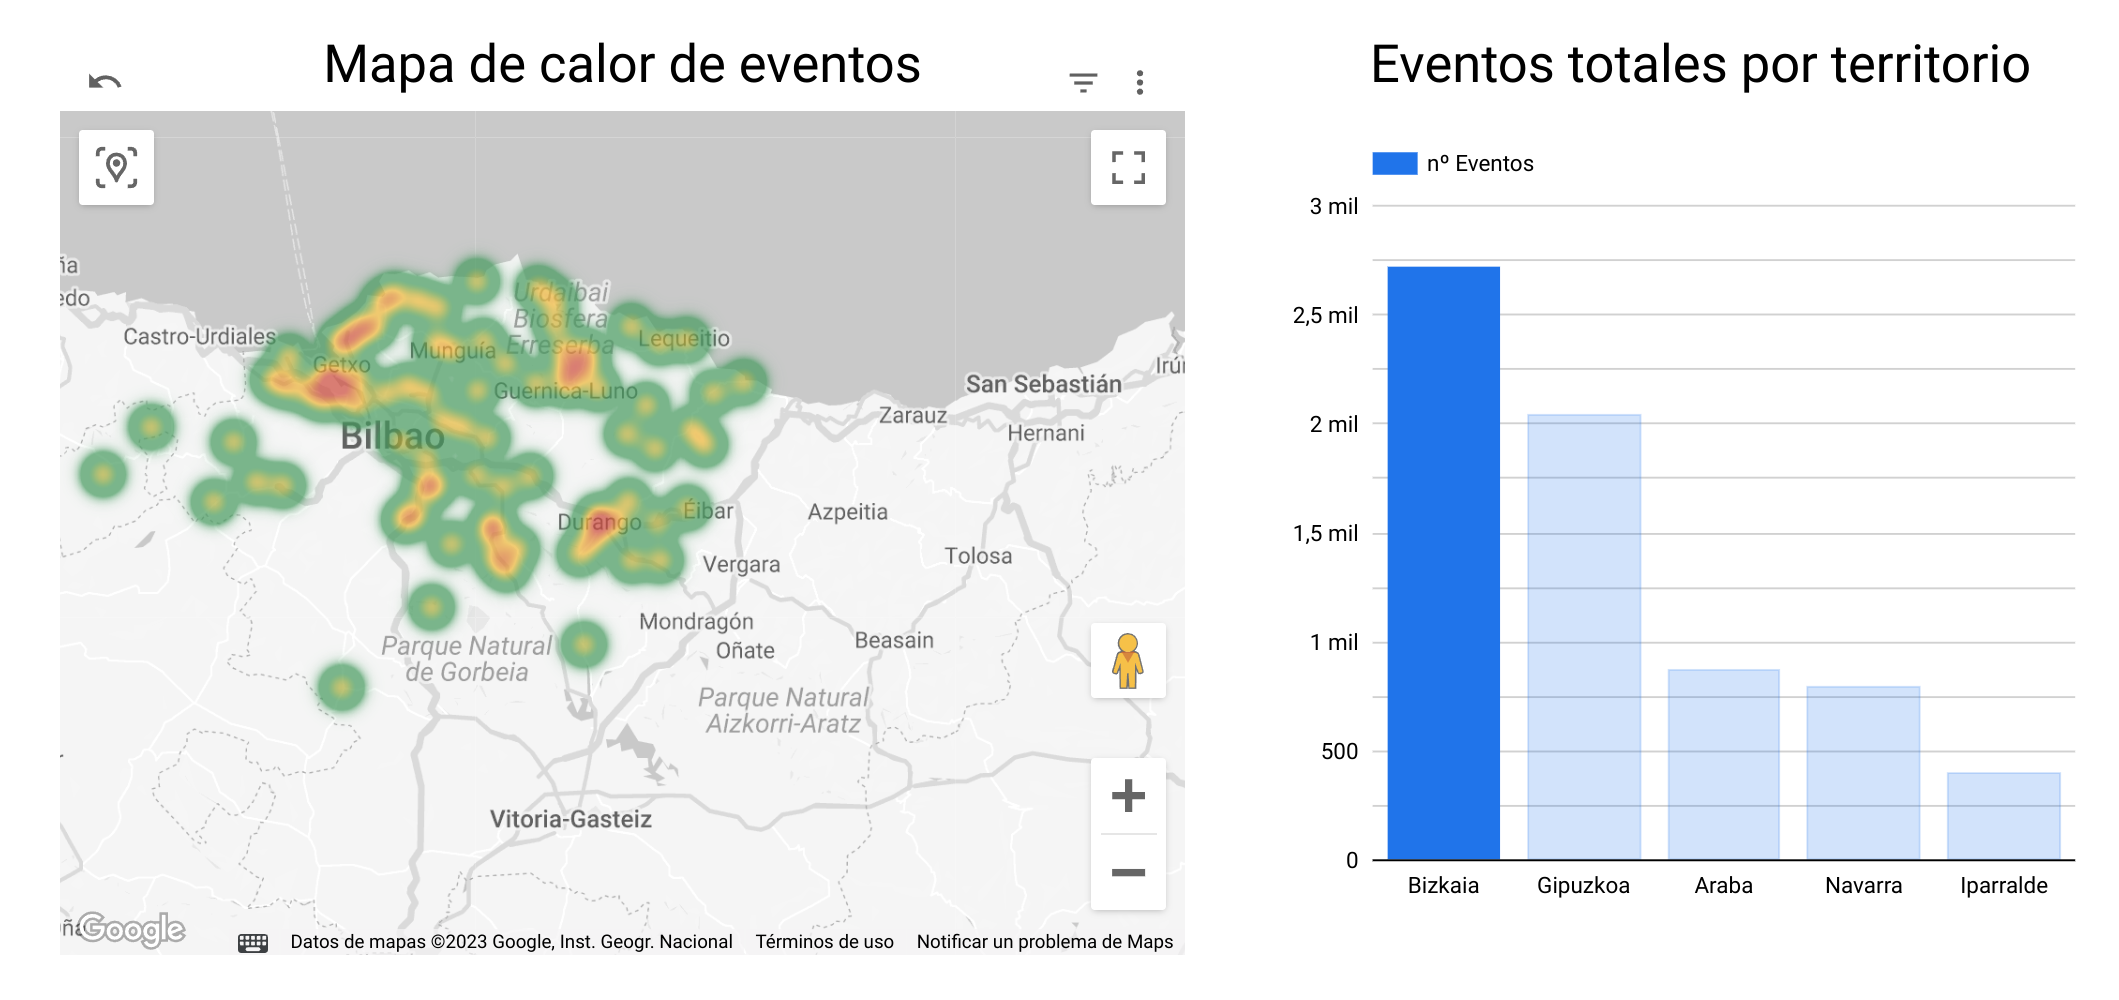
\includegraphics[frame,width=0.9\linewidth]{graficos.png}
        \captionof{figure}{Gráficos enlazados}
    \end{center}

    \item Se pueden generar \textbf{filtros} para realizar una búsqueda en los datos.

    \item Podemos \textbf{compartir} el dashboard creado o generar una presentación.

\end{itemize}


Como contrapartida, también pueden existir algunos inconvenientes a la hora de utilizarlos, que debemos de tener claros antes de utilizarlos:

\begin{itemize}
    \item Estamos \textbf{limitados a las características que ofrecen}. Por lo tanto, si nos interesa crear un gráfico distinto a los que ofrece, no vamos a poder hacerlo.

    \item Los datos deben de estar en el \textbf{formato que acepte la herramienta}. Si programamos nosotros, el formato puede ser propio, o el diccionario de datos puede estar a nuestro gusto.

    \item \textbf{Dependencia} de la herramienta. Si deciden eliminar funcionalidades, hacerla de pago, ... deberemos migrar los datos y crear de nuevo el panel.

\end{itemize}


\chapter{Entendiendo los datos}

Antes de crear un panel de información debemos tener claro los tipos de datos que tenemos, cómo están organizados (o si debemos organizarlos), en qué formato están, ... es por eso que debemos realizar un análisis previo de los mismos.

\section{Análisis de datos}

A la hora de realizar el análisis de datos, debemos tener en cuenta, al menos, las siguientes características:

\begin{itemize}
    \item \textbf{Fuente de los datos}: ¿son datos propios? ¿podemos recuperarlos en cualquier momento? ¿son fiables?

    \item \textbf{Formato de los datos}: Debemos tener en cuenta no sólo el formato del fichero en el que obtenemos los datos, si no si estos están normalizados. Por ejemplo, si los números están guardados en formato entero/real o en formato texto; si existen datos de geolocalización, si están separados o agregados; ...

    \item \textbf{Entender los datos}: Aunque pueda parecer obvio, es necesario \textbf{entender cada apartado de los datos} para posteriormente relacionarlos entre sí, y para hacer uso de ellos en el panel/gráfico.
\end{itemize}


\section{Creación del esquema de datos}
Teniendo en cuenta el punto anterior, quizá sea necesario normalizar los datos o crear un formato específico. Por lo tanto, debemos de conocer algún tipo de herramienta o de lenguaje de programación que nos permita hacerlo.

Si los datos en bruto obtenidos no cumplen las expectativas, entre las tareas que debemos realizar estarán:

\begin{itemize}
    \item \textbf{Normalizar los datos}: A cada tipo de datos convertirlo al formato que debe ser.
    \item \textbf{Diccionario de datos}: Crear el esquema/diccionario de datos que mejor se adecúe a los datos y al sistema de panel que vayamos a utilizar.

\end{itemize}

\section{Crear el tipo de fichero}
Por útlimo, será necesario generar el tipo fichero con el formato que la herramienta necesita: json, CSV, formato excel, ...

Para ello, dependiendo del esquema de datos, podremos generar el fichero con herramientas simples (por ejemplo excel, para generar un fichero en formato CSV) o deberemos hacer uso quizá de lenguajes de programación con librerías específicas que nos faciliten la labor (por ejemplo python).

\section{Documentación del análisis}
Siempre es recomendable documentar el proceso del análisis de datos para entender en etapas sucesivas, o tiempo después, el por qué se han modificado los datos tal como se ha hecho, o la razón de hacer uso de un tipo de fichero y no otro.

La documentación también facilitará el realizar modificaciones más adelante o para poder realizar adaptaciones a nuevas herramientas. De esta manera, en principio, tendremos parte del trabajo hecho y no habrá que volver a realizarlo.

\chapter{Looker Studio como generador de paneles de información}

\href{https://lookerstudio.google.com/}{Looker Studio}, anteriormente conocida como DataStudio, es una herramienta de Google para visualizar y crear paneles informativos con datos que proporcionamos desde distintas fuentes.

Es una herramienta gratuita, fácil de usar y que permite generar distintos tipos de paneles con los datos proporcionados. Aparte, también permite crear otros tipos de visualizaciones, por lo que la comunidad aporta nuevos \href{https://lookerstudio.google.com/visualization}{paneles}.

